%%%%%%%%%%%%%%%%%%%%%%%%%%%%%%%%%%%%%%%%%%%%%%%%%%%%%%%%%%%%%%%%%%%%%%%%%%%%
% AGUtmpl.tex: this template file is for articles formatted with LaTeX2e,
% Modified July 2014
%
% This template includes commands and instructions
% given in the order necessary to produce a final output that will
% satisfy AGU requirements.
%
% PLEASE DO NOT USE YOUR OWN MACROS
% DO NOT USE \newcommand, \renewcommand, or \def.
%
% FOR FIGURES, DO NOT USE \psfrag or \subfigure.
%
%%%%%%%%%%%%%%%%%%%%%%%%%%%%%%%%%%%%%%%%%%%%%%%%%%%%%%%%%%%%%%%%%%%%%%%%%%%%
%
% All questions should be e-mailed to latex@agu.org.
%
%%%%%%%%%%%%%%%%%%%%%%%%%%%%%%%%%%%%%%%%%%%%%%%%%%%%%%%%%%%%%%%%%%%%%%%%%%%%
%
% Step 1: Set the \documentclass
%
% There are two options for article format: two column (default)
% and draft.
%
% PLEASE USE THE DRAFT OPTION TO SUBMIT YOUR PAPERS.
% The draft option produces double spaced output.
%
% Choose the journal abbreviation for the journal you are
% submitting to:

% jgrga JOURNAL OF GEOPHYSICAL RESEARCH
% gbc   GLOBAL BIOCHEMICAL CYCLES
% grl   GEOPHYSICAL RESEARCH LETTERS
% pal   PALEOCEANOGRAPHY
% ras   RADIO SCIENCE
% rog   REVIEWS OF GEOPHYSICS
% tec   TECTONICS
% wrr   WATER RESOURCES RESEARCH
% gc    GEOCHEMISTRY, GEOPHYSICS, GEOSYSTEMS
% sw    SPACE WEATHER
% ms    JAMES
% ef    EARTH'S FUTURE
% ea    EARTH AND SPACE SCIENCE
%
%
%
% (If you are submitting to a journal other than jgrga,
% substitute the initials of the journal for "jgrga" below.)

\documentclass[draft,ras]{agutex}
\usepackage{graphicx}   
\usepackage{setspace}
\usepackage{amsxtra}
\usepackage{amsmath}
\usepackage{amssymb}
\usepackage{multirow}
\usepackage{bm}
\RequirePackage{lineno}
\linenumbers
% graphics path
\graphicspath{{Figs/}}

% Author names in capital letters:
\authorrunninghead{Swoboda ET AL.}

% Shorter version of title entered in capital letters:
\titlerunninghead{ISR ERRORS}

%Corresponding author mailing address and e-mail address:
%\authoraddr{Corresponding author: A. B. Smith,
%Department of Hydrology and Water Resources, University of
%Arizona, Harshbarger Building 11, Tucson, AZ 85721, USA.
%(a.b.smith@hwr.arizona.edu)}

\begin{document}

%% ------------------------------------------------------------------------ %%
%
%  TITLE
%
%% ------------------------------------------------------------------------ %%


%\title{Trade-Offs Between Statistical Accuracy and Space-Time Resolution in ISR}
\title{Observability of Ionospheric Space-Time Structure with ISR:   A simulation study }
%%%%%%%%%%%%%% Author Info %%%%%%%%%%%%%%%%%%%%%%%%%%%%%%%%%%%%%
\authors{John Swoboda,\altaffilmark{1}
Joshua Semeter,\altaffilmark{1} Matthew Zettergren,  \altaffilmark{2} Philip Erickson, \altaffilmark{3}}

\altaffiltext{1}{Department of Electrical \& Computer Engineering,
Boston University, Boston, Massachusetts, USA.}
\altaffiltext{2}{Physical Sciences Department, Embry-Riddle Aeronautical University, Daytona Beach, Florida, USA.}
\altaffiltext{3}{Haystack Observatory, Massachusetts Institute of Technology, Westford, Massachusetts, USA.}
%%%%%%%%%%%%%% Abstract %%%%%%%%%%%%%%%%%%%%%%%%%%%%%%%%%%%%%
%% ------------------------------------------------------------------------ %%
%
%  ABSTRACT
%
%% ------------------------------------------------------------------------ %%

% >> Do NOT include any \begin...\end commands within
% >> the body of the abstract.

\begin{abstract}
As with any sensing modality, incoherent scatter radar (ISR) has inherent errors and uncertainty in its measurements. A number of theoretical aspects behind these errors have been documented in the literature. The main sources of this error comes from spatiotemporal ambiguities and statistical errors that arise from the inherent fluctuation of the medium. 

From the point of view from an experiment designer these sources of error can lead to a trade off between spatial and temporal resolution and statistical accuracy. The designer then has to work with questions dealing with resource allocation, such as how long to dwell in a specific direction. These questions can be rather hard to solve because there are a large number of degrees of freedom when designing an experiment.

With the recent application of phased array antennas with pulse to pulse steering, the number of degrees of freedom in experiment design have exploded. These types of systems, like AMISR and EISCAT-3D, allow for greater flexibility in processing along with making it is now possible to create full volumetric reconstructions of plasma parameters. These phased array systems are used heavily in the high latitude region of the ionosphere, which can have plasma phenomena that is highly variable in space and time. In order to develop an experiment to observe the plasma phenomena researchers have to wade through a number of different trade offs. To understand all of these trade offs may need to simulate the experiment.

This publication will show a simulator that can take a field of plasma parameters and create ISR data at the IQ level and then process it to show a possible reconstruction of the parameters field. It can give researchers a new tool that can assist them in the set up their experiments. To show the utility of the simulator for experiment design for one of the examples we will data from a self-consistent multi-ionic fluid transport model. This will demonstrate the impact the forward model of the ISR and give an example of how to iterate through different simulation set ups. 

\end{abstract}

%% ------------------------------------------------------------------------ %%
%
%  BEGIN ARTICLE
%
%% ------------------------------------------------------------------------ %%

% The body of the article must start with a \begin{article} command
%
% \end{article} must follow the references section, before the figures
%  and tables.

\begin{article}

\section{Introduction}
Incoherent scatter radar is an important diagnostic for the ionosphere in that it can give direct measurements of the intrinsic plasma parameters  \citep{dougherty:farley1960, farleydougherty:ISR2, doughteryfarley:ISR3, hagfors1961}. As with all diagnostic tools it has associated with it sources of errors which include time and spatial ambiguities \citep{farley1969, farleycomppower1969, hysell2008, RDS:RDS20236}.  

One unique aspect of ISR is that inherent random fluctuations of the plasma are used to create these measurements. These fluctuations are used by creating second order statistics from a scattered signal, specifically an autocorrelation function (ACF) \citep{farley1969}. The statistical nature of the target itself yields the requirement of averaging numerous realizations of the ACF to reduce the variance of the estimate. This forces the assumption of stationarity for a space-time cell, which may not be true. In the end this creates a trade-off between space-time resolution and the variance of the measurements.

Application of electronically steerable array (ESA) technology to ISR has been a recent advancement for the community. ISRs such as these, like the Advanced Modular Incoherent Scatter (AMISR) systems, have already been deployed in Poker Flat Alaska and Resolute Bay Canada \citep{Nicolls:2007ie, dahlgren2012di}. These ESA based systems are seen as the future of the ISR sensor modality due to the flexibility in beam steering, processing and other aspects over dish based systems. The next step in the evolution of these systems is expected to be the EISCAT-3D project, which will have a number of enhancements such as multi-static processing capability and be able to receive and process data from each phased array element by default.

One benefit of ESA based ISR is that volumetric reconstructions of plasma parameters can be created \citep{Semeter2009738, Nicolls:2007ie, dahlgren2012di}. These systems also have ben used to reconstuct full vector parameters using estimates of the ion velocity which can be determined using the Doppler shift of spectra \citep{butler:imagingfregiondrifts,RDS:RDS20195}. Still it has been shown that the volumetric reconstructions can yield measurements with a high degree of ambiguity \citep{Dahlgren:2012dq}. Similar type of ambiguities have been seen when using systems with a dish antenna as well. In \citet{Semeter:2005fo} the authors to show an undersampling in the horizontal dimension, but are able to compensate by changing processing parameters.

With these new capabilities for the ISR community a discussion of the possible sources of uncertainty and error is needed. These sources of error and ambiguity though are difficult understand in the context of experiment design. With that in mind it may be useful to simulate the ISR measurement process before an experiment is attempted. With that in mind this paper will show how one could simulate an experiment, the outline of this is a follows. After listing the possible sources of error and ambiguity in ISR our simulation method will be detailed. After which  a number of examples of the simulator will be shown. These example range from a stationary column of enhanced electron density to the output of a self-consistent multi-fluid ionosphereic model \citep{semeter:plasmatransport2012}. These examples will illustrate how one could develop their experiments in a systematic way in order make measurements that best reflect the physics present in the ionosphere.
%%%%%%%%%%%%%%%%%%%%%%%%%%%%%%%%%%%%%%%%%%%%%%%%%%%%%%%%%%%%%%%%%%%%%%%%%%%%%%%%%%%%%%%%%%%%%%
\section{ISR Errors}

In this section the main sources of ISR errors will be discussed. The first part of this discussion will cover the statistical errors that arise from the ISR process. After that the errors from the spatial and temporal ambiguity of ISR systems will be shown. This in the end will lead to trade offs that the experiment designer will have to face.

\subsection{Statistical Errors}

To measure the plasma parameters ISR takes advantage of the random fluctuations of electron density in the ionosphere. The theory of how the plasma parameters impact the statistics of these fluctuations have been discussed since the first use of this sensor modality \citep{gordon58,dougherty:farley1960, farleydougherty:ISR2, doughteryfarley:ISR3, hagfors1961}, and even as recent as 2011 there have been new formulations of this theory \citep{kudeki:milla:1,kudeki:milla:2}. 

The two main sources of statistical error will covered here are the random fluctuations from the electron density and noise from within the sensor itself. There are other sources of statistical error including sky noise and coherent scatter from other targets. 

The raw incoherent scatter signal is itself is a random process. As such it is necessary to average samples of an estimator for autocorrelation or spectrum \citep{Diaz:2008co}. An easy rule of thumb to understand how the error will reduce can be seen in \citet{farley1969},

\begin{equation}
\label{eqn:basicerror}
\left\langle \left| \hat{R}(\tau) -R(\tau) \right|^2 \right\rangle \propto \frac{1}{\sqrt{J}},
\end{equation}
\noindent where $R(\tau)$ is the ACF as a function of lag $\tau$, $\hat{R}(\tau)$ is its estimate and $J$ is the number of samples or pulses averaged together to create the estimate. 

The variance of this signal is further degraded once noise from the sensor is added. The noise from the sensor is assumed to be uncorrelated to the signal. Thus the error from the noise can simply be added to the error from the inherent fluctuations in the signal. 

\subsection{Space-Time Errors}

The errors created through the ambiguity function lead to a blurring or averaging of ACFs from different points in time and space. This is similar to a blurring operator one might see in a camera or numerous other types of sensors. With ISR this can be more problematic due to the non-linear fitting step.

The space-time ambiguity, $L(\tau_s,\mathbf{r}_s,t_s,\tau,\mathbf{r},t)$, is the kernel of Fredholm integral equation of the first kind operating on the ACF, $R(\tau,\mathbf{r},t)$, which can change over space, $\mathbf{r}$, and time $t$. which can be represented as follows,

 \begin{equation}
  \label{eqn:staf}
  \rho(\tau_s,\mathbf{r}_s,t_s) =\int L(\tau_s,\mathbf{r}_s,t_s,\tau,\mathbf{r},t)R(\tau,\mathbf{r},t)dVdtd\tau,
\end{equation}

\noindent where the subscript $s$ represents the same variable but now discretely sampled by the radar. 

The kernel is a separable function when the spatial coordinates are spherical, where ($r,\theta,\phi)$ represent, range, azimuth and elevation respectively. This the changes Equation \ref{eqn:staf} as follows,

\begin{equation}
\label{eqn:stafbrok}
\rho(\tau_s,\mathbf{r}_s,t_s)= \int G(t_s,t)F(\theta_s,\phi_s,\theta,\phi)W(\tau_s,r_s,\tau,r) R(\tau,\mathbf{r},t) dVdt d\tau,
\end{equation}

\noindent where $G(t_s,t)$ is the kernel for the time dimension, $F(\theta_s,\phi_s,\theta,\phi)$ is radar beam shape which acts as a kernel in azimuth and elevation, and $W(\tau_s,r_s,\tau,r) $ which is the range ambiguity function which acts as a kernel along range $r$ and lag $\tau$. The derivation of this operator can be seen in \citet{RDS:RDS20236}.

These two sources of error create a significant trade off between statistical variation of the signal and spatial and temporal resolution of the signal. In order to reduce the statical fluctuations in the signal pulses need to be averaged together. This is necessary even for the case where there is no noise, in a sense the infinite signal to noise ratio (SNR) case. This integration is mainly done over time but can be done over space as well. For phased array systems this mixture of spatial and temporal averaging can be done by averaging together beams. This though will reduce cross range resolution but could possibly improve temporal resolution. It is for this reason these types of trade offs can best be explored through simulation, which will be covered in the following sections.
 %%%%%%%%%%%%%%%%%%%%%%%%%%%%%%%%%%%%%%%%%%%%%%%%%%%%%%%%%%%%%%%%%%%%%%%%%%%%%%%%%%%%%%%%%%%%%
\section{Simulator}

The following section will detail the processing steps in the ISR simulator. The simulator allows one to analyze different experiment scenarios by implementing the ISR measurement process with the error from both from both space-time ambiguity and the statistical error. The space-time ambiguity is modeled using a coordinate transform and the the pulse as a windowed and the statistical error is taken into account by creating complex shaped Gaussian noise. The first part will detail the how filters are created to make the noise. The next one will cover creation of the in-phase and quadrature data (IQ data). The last portion will detail the processing used to create the estimates of the ACFs, which will also be referred to as lag products.

\subsection{Creating Filters}

The simulator takes as input a discretized set of ionosphere parameters in Cartesian coordinates, which change with time. The first step in the simulator will be from each set of parameters an ISR spectrum is calculated, Thus for each point in time in space for the simulator there will be an intrinsic ISR spectrum. For details on creating these spectra see \citet{kudeki:milla:1} and \citet{kudeki:milla:2}. 

Once the spectra have been created the simulator changes to a spherical coordinate system. This coordinate change acts as a linear operator in the spatial dimensions as the spectra are weighted and averaged. The weighting in azimuth and elevation is determined by the antenna beam pattern while the weighting in range is simply just a test of whether the spectra are with in the range gate. If there are no spectra within the range gate a nearest neighbor rule is used which selects the closest point in Cartesian space. This method to create the spectra for each point is an acceptable approximation because spatial correlations between the electron density fluctuations will be on the order of the Debye length \citep{farley1969}, which is significantly smaller than the beam width or range gate size. The entire process of the spatial sampling is shown in the simplified diagram in Figure \ref{fig:beamdia}.

\begin{figure}[!t]
\centering
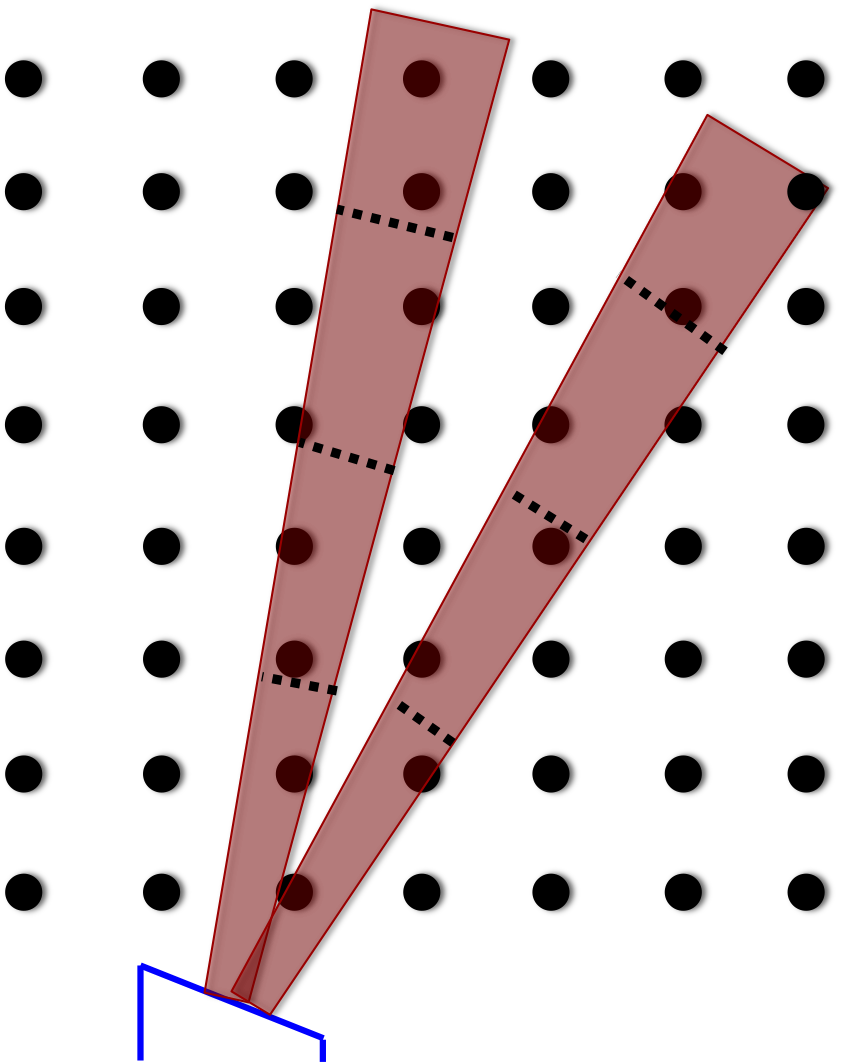
\includegraphics[width=2in]{beamsampling}
\caption{Beam Sampling Diagram}
\label{fig:beamdia}
\end{figure}
 
% Once the spectrum at the specific point in range and angle space has been determined, the filter $H_m(\omega)$, is created by simply taking the square root of the spectrum, $S_m(\omega | \: \bm{\theta})$,

% \begin{equation}
% \label{eq1}
% H_m(\omega) = \sqrt{S_m(\omega | \: \bm{\theta})}.
% \end{equation}

Once the spectrum at the specific point in range and angle space has been determined, the filter is created. The method to create the filter given a desired spectrum or ACF can be done in a number of ways \cite{Kasdin:1995wi}. The current implementation in the simulator creates an infinite impulse filter. The coefficients are determined using the ACF by solving the following set of equations,

\begin{equation}
\label{eq:filtereq}
\begin{bmatrix} R_m(0) & R_m(1)& \cdots & R_m(L-1) \\ R_m(L-1) & R_m(0)& \cdots & R_m(L-2)\\ \vdots & &\ddots  & \vdots \\  R_m(1) & R_m(2) & \cdots & R_m(0) \end{bmatrix} \left[ \begin{array}{c} a_1\\ a_2\\\vdots \\ a_L \end{array} \right]=\left[ \begin{array}{c} R_m(1) \\ R_m(2)\\ \vdots \\R_m(L) \end{array} \right]
\end{equation}

\noindent where $R_m(l)$ are the ACF values, $L$ is the desired length of the filter, and $ a_i$ are the set of filter coefficients. The filter then takes the form in the frequency domain as the following,

\begin{equation}
\label{eq:filtz}
H_m(z) = \frac{G}{1-\displaystyle \sum_{l=1}^{L} a_l z^{-l}}.
\end{equation}
\noindent The gain term $G$ is used to make sure the noise is the correct variance. This can be calculated as 

\begin{equation}
\label{eq:gainterm}
G=\sqrt{\displaystyle \sum_{l=0}^L -a_l R_m(l)},
\end{equation}

\noindent where $a_0=-1$. 
%\noindent The term $ \bm{\theta}$ refers to the plasma parameters needed to make the spectrum. This filter then is used to create the synthetic IQ data.

\subsection{ IQ Data Creation}
The basic idea behind creating the IQ data is to take a complex white Gaussian noise process and shape the spectrum of its output using a filter. As seen in the previous subsection, each point in space and time will have a separate noise plant and filter which is derived from the plasma and radar parameters parameters, like that seen in Figure \ref{fig:IQdiagram}. 

\begin{figure}[h!]
\centering
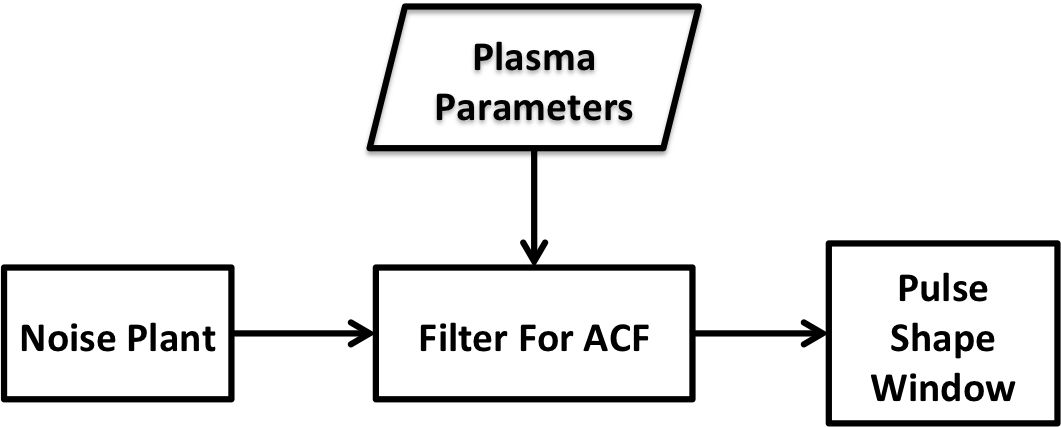
\includegraphics[width=4in]{diagrampart}
\caption{Diagram for I/Q simulator signal flow.}
\label{fig:IQdiagram}
\end{figure}

The creation of one set of IQ data using a CWGN, ($w(k)\sim CN(0,\mathbf{I})$) can be represented as the following:   

\begin{equation}
\label{eq2}
y_m (k)= s(k)\left[h_m(k)*w(k)\right],
\end{equation}
 
\noindent where $s(k)$ is the pulse shape. The pulse shape acts as a window, as the plasma will only reflect energy during the time it is illuminated. The application of this filter is actually done in the frequency domain. This is possible because the Discrete Fourier Transform (DFT) of a vector of CWGN is also CWGN. The only difference is that there is a change in the variance, which is tied to the number of points used in the DFT \citep{kayvol1}. With this in mind Equation \ref{eq2} can be implemented as the following,

\begin{equation}
\label{eq:fftfilt}
y_m (k)= s(k)\displaystyle \sum_{i=0}^{K-1}e^{j\omega_ik}\left[ \sqrt{S_m(\omega_i | \: \bm{\theta})}w(\omega_i)\right],
\end{equation}

\noindent where $\omega_i$ is the frequency variable, $w(\omega_i) \sim CN(0,\mathbf{I})$ and $K$ is the number of points used for the DFT \citep{michellnoisesim1981}.

\begin{figure}[!h]
\centering
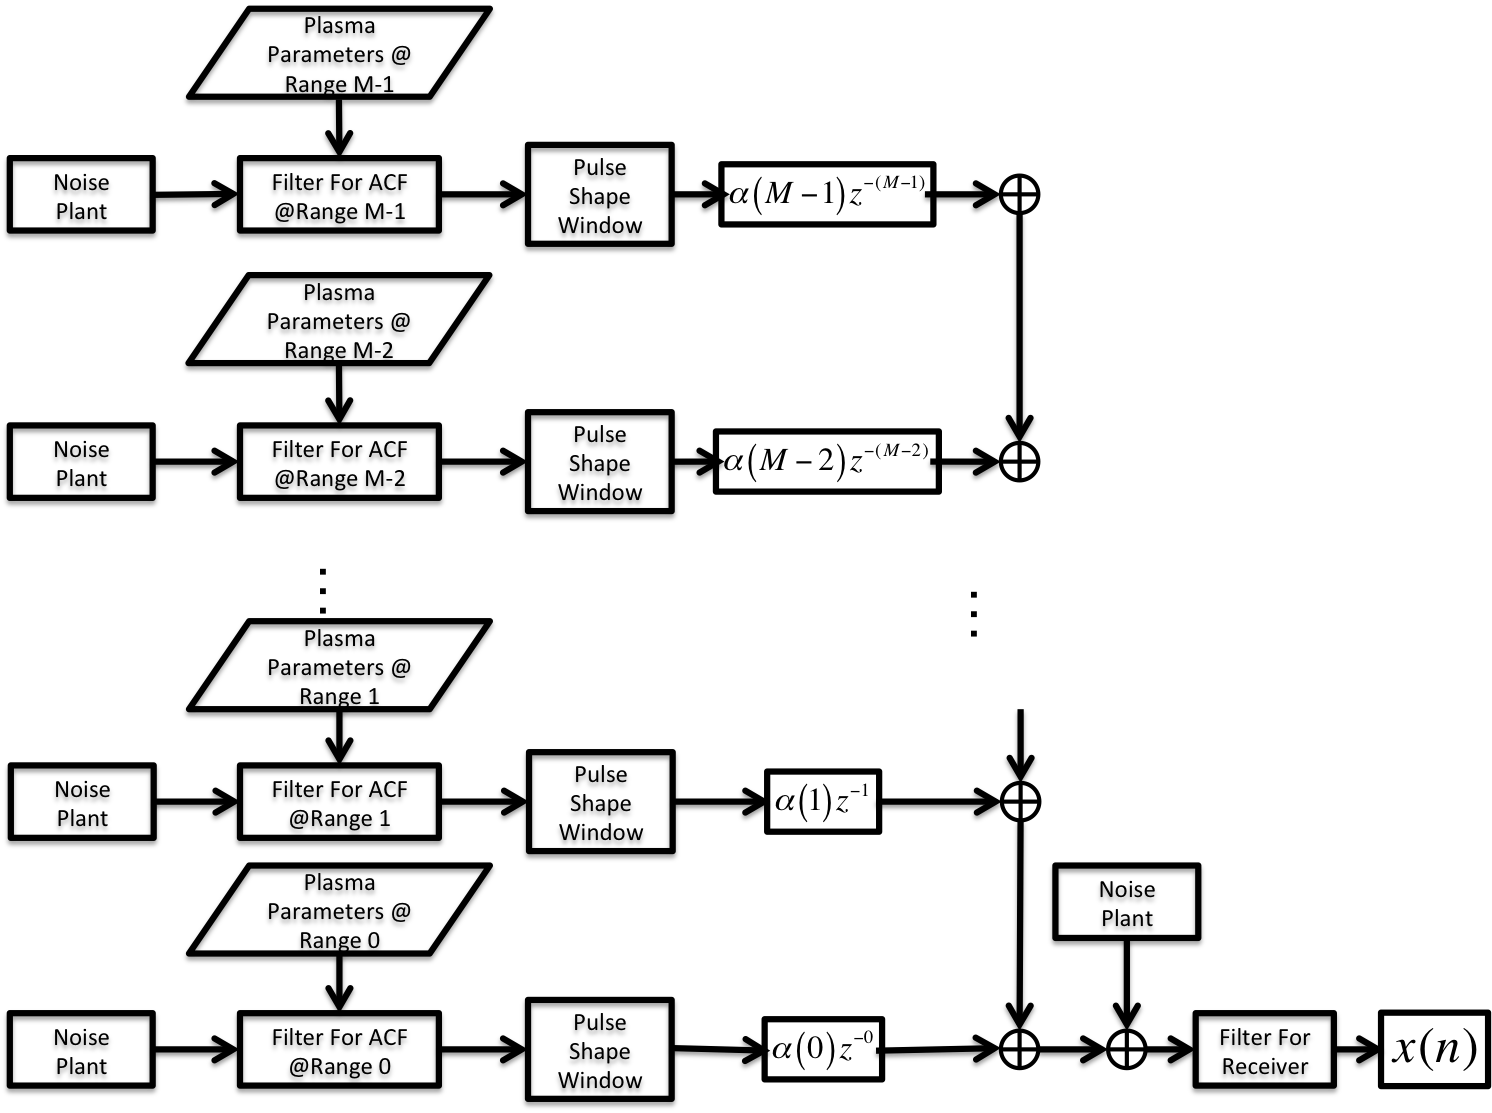
\includegraphics[width=7.0in]{diagram}
\caption{ISR Simulation Diagram}
\label{fig:isrdiag}
\end{figure}


After the data for each range gate $y_m(k)$ is created the power of the return is calculated

\begin{equation}
\label{eq3}
P_r = \frac{cG \lambda^2}{2(4\pi)^2}\frac{P_t }{R^2}\frac{\sigma_e N_e}{(1+k^2\lambda_D^2),(1+k^2\lambda_D^2 + T_r)}
\end{equation}
 
 \noindent where $P_r$ is the power received, $c$ is the speed of light, $G$ is the gain of the antenna, $P_t$ is the power of the transmitter, $\sigma_e$ is the electron radar cross section, $k$ is the wavenumber of the radar, $\lambda_D$ is the Debye length, $N_e$ is the electron density and $T_r$ is the electron to ion temperature ratio.
  
Once the power has been calculated for each range all of the data is delayed and summed together so as to model the arrival of the radar return at the receive: 
 
\begin{equation}
\label{eq4}
x(n) = \displaystyle\sum\limits_{m =0}^{M-1} \alpha(m)y_m(n-m),
\end{equation}

\noindent where $\alpha(m) = \sqrt{P_r(m)}/\hat{\sigma_y}$ and $\hat{\sigma_y}$ is the estimate of the standard deviation of $y_m(k)$. Lastly, to model the inherent noise in the radar and environment more complex Gaussian noise is added

\begin{equation}
\label{eq:addnoise}
x_f(n) = x(n) +\sqrt{\frac{k_bT_{sys}B}{2}} w(n), \quad w(n)\sim CN(0,1)
\end{equation}

\noindent where $k_b$ is Boltzmann's constant, $T_{sys}$ is the system temperature and $B$ is the system bandwidth.
A full diagram of the model can be seen in Figure \ref{fig:isrdiag}.


\subsection{ACF Estimation}

After the IQ data has been created it is processed to create estimates of the ACF at desired points of space. This type of processing has been detailed and analyzed in \citep{farley1969} and in other publications. This processing follows a flow chart seen in Figure \ref{fig:chain}.

\begin{figure}[!t]
\centering
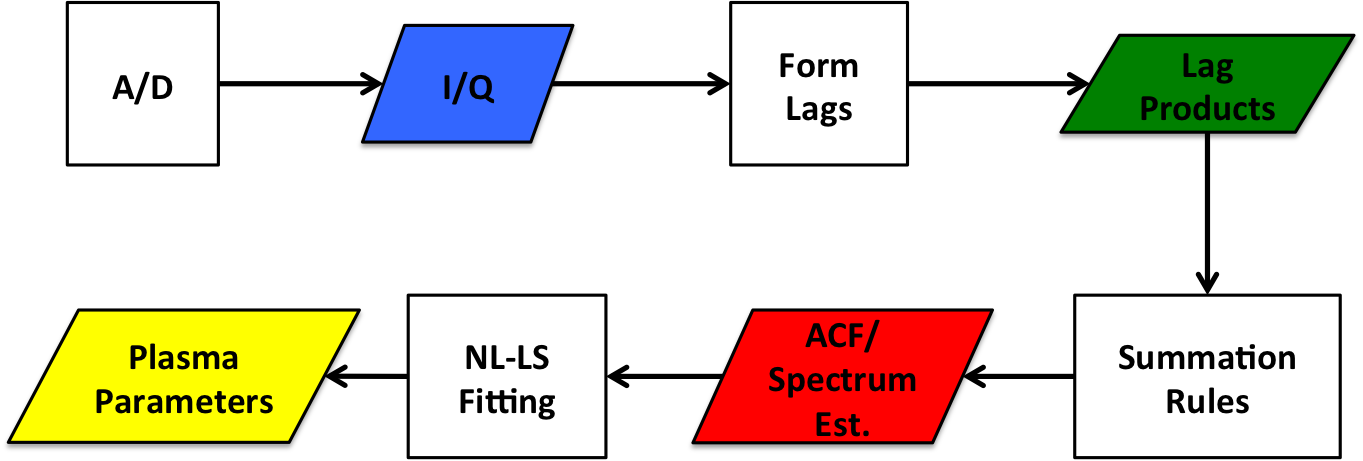
\includegraphics[width=6in]{datastackchain}
\caption{ISR signal processing chain, with signal processing operations as squares and data products as diamonds.}
\label{fig:chain}
\end{figure}


The lag product formation is an initial estimate of the autocorrelation function. The sampled I/Q can be represented as $x(n) \in\mathbb{C}^N$ where $N$ is the number of samples in an inter pulse period. For each range gate $m\in 0,1,...M-1$ an autocorrelation is estimated for each lag of $l \in 0,1...,L-1$.  To get better statistics this operation is performed for each pulse $j\in 0,1,...J-1$ and then summed over the $J$ pulses. The entire operation to form the initial estimate of $\hat{R}(m,l)$ can be seen in Equation \ref{eq:lagpro}:

\begin{equation}
\label{eq:lagpro}
\hat{R}(m,l) = \displaystyle\sum\limits_{j=0}^{J-1} x(m-\lfloor l/2\rfloor,j)x^*(m+\lceil l/2 \rceil,j).
\end{equation}

The case shown in Equation \ref{eq:lagpro} is a centered lag product, other types of lag products calculations are available but generally a centered product is used. In the centered lag product case range gate index $m$ and sample index $n$ can be related by $m=n-\lfloor L/2\rfloor$ and the maximum lag and sample relation is $M=N-\lceil L/2 \rceil$.  This lag product formation is the first step in taking a discrete Wigner Distribution \citep{TFAcohen}.

This specific type of lag product formation is detailed in \citep{farley1969} and had been referred to as unbiased. This terminology does differ from what is used in statistic signal processing literature such as \citep{randomsigshanmugan} where the unbiased autocorrelation function estimate is carried out as so,

\begin{equation}
\label{eq:lagproub}
\hat{R}(m,l) = \frac{1}{L-l}\displaystyle\sum\limits_{j=0}^{J-1} x(m-\lfloor l/2\rfloor,j)x^*(m+\lceil l/2 \rceil,j).
\end{equation}

\noindent With out the $\frac{1}{L-l}$ term the estimator will be windowed with a triangular function thus impacting the estimate of the ISR spectrum as this will act as a convolution in the frequency domain. This bias is taken into account in \citep{farley1969} but it is simply wrapped up into the ambiguity function. 

Applying a summation rule is generally the next step in creating an estimate of the autocorrelation function.  This is done to get a constant range ambiguity across all of the lags for long pulse experiment\citep{nygren1996}. It also equalizes the statistics for each lag, as the number of samples for each lag in Equation \ref{eq:lagproub} decreases.  An example summation rule for a central product is shown in Figure \ref{fig:sumrule}. In the figure the image on the left is a basic representation of an ambiguity function of a long pulse.  Its mirrored on the right with red bars which would show the integration area under it so the ambiguity function for each lag will be of equal size in range. There are a number of different summing rule each with their own trade offs \citep{nygren1996}.

%In the processing this is basically a summing of lags from different ranges. The amount of summing is similar to what is shown in Figure \ref{fig:sumrule}.   

Lastly an estimate of the noise correlation is subtracted out of $\hat{R}(m,l)$, which is defined as $\hat{R}_w(m,l)$:

\begin{equation}
\label{eq:lagpronoise}
\hat{R}_w(m,l) = \displaystyle\sum\limits_{j=0}^{J-1} w(m_w-\lfloor l/2\rfloor,j)w^*(m_w+\lceil l/2 \rceil,j),
\end{equation}

\noindent where $w(n_w)$ is the background noise process of the radar.  Often the noise process is sampled during a calibration period for the radar when nothing is being emitted.  The final estimate of the autocorrelation function after the noise subtraction and summation rule will be represented by $\hat{R}_f(m,l)$.
\begin{figure}[!t]
\centering
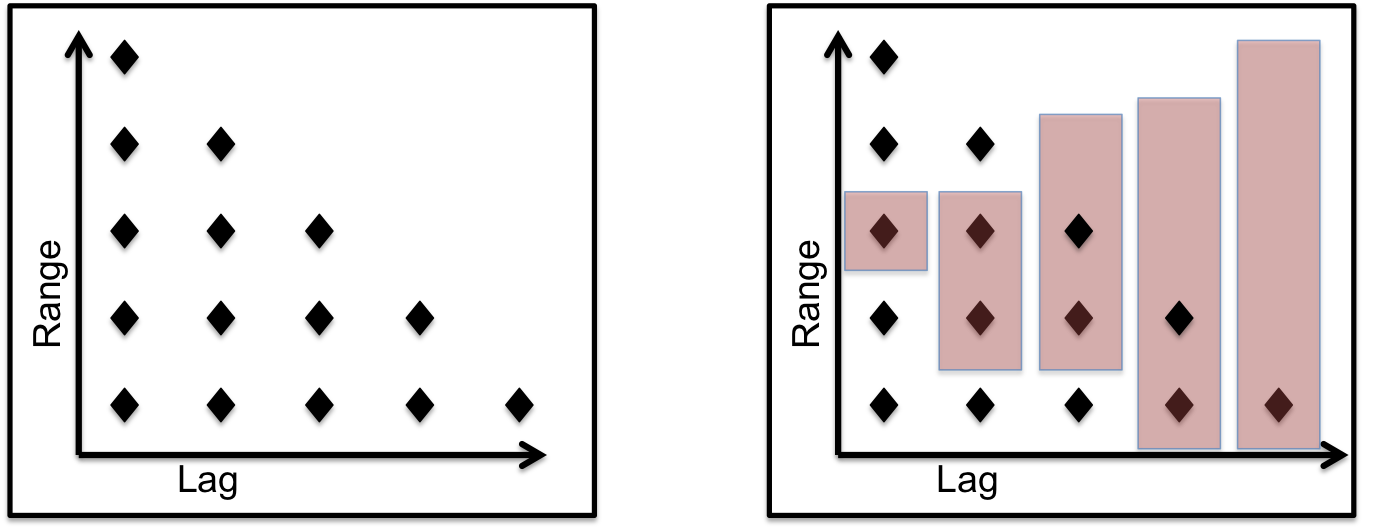
\includegraphics[width=3in]{sumrule}
% where an .eps filename suffix will be assumed under latex, 
% and a .pdf suffix will be assumed for pdflatex; or what has been declared
% via \DeclareGraphicsExtensions.
\caption{Summation Rule Diagram}
\label{fig:sumrule}
\end{figure}

After the final estimation of the spectrum is complete the nonlinear least squares fitting takes place to determine the parameters.  The basic class of nonlinear least-squares problems as seen in \citep{kayvol1}, are shown in Equation \ref{nlls},

\begin{equation}
	\hat{\mathbf{p}}= \underset{\mathbf{p}}{\text{argmin}} (\mathbf{y}-\bm{\theta}(\mathbf{p}))^*\bm{\Sigma}^{-1}(\mathbf{y}-\bm{\theta}(\mathbf{p})).
\label{nlls}
\end{equation}

In Equation \ref{nlls}, the data represented as $\mathbf{y}$ would be the final estimate of the autocorrelation function $\hat{R}_f(m,l)$ at a specific range or its spectrum $\hat{S}_f(m,\omega)$.  The parameter vector $\mathbf{P}$ would be the plasma parameters $N_e$, $T_e$, $T_i$ and various other parameters including ion velocities. The fit function $\bm{\theta}$ is the IS spectrum calculated from models, such as once seen in \citep{kudeki:milla:1}, smeared by the ambiguity function.  In the case of the long pulse the ambiguity can be simply applied by multiplying it with the autocorrelation function $R(l)$, if the summation rule is properly applied. 

%The correlation matrix $\bm{\Sigma}$ is often realized as a diagonal matrix for many ISR systems the variance of the lags or each point of the spectrum being the values. The variance of the ACF estimator can be estimated using the following,
%
%\begin{equation}
%\label{eqn:acfvar}
%\sigma_{\hat{R}(l)}^2=\frac{1}{JL}\displaystyle \sum_{m=-(L-l-1)}^{L-l-1}\left(\frac{L-|m|+1}{L}\right)\left(|\hat{R}(m)|^2 +|\hat{R}(m+l)\hat{R}(m-l)|\right) + \hat{N}^2
%\end{equation}
%
%\noindent where $N$ is the estimated noise power. To estimate the spectrum variance the matrix $\bm{\Sigma}$ is transformed in to the Fourier domain using FFTs (FFT on the columns and IFFT on the rows) so as to model the $\mathbf{F}\bm{\Sigma} \mathbf{F}^*$ matrix operation. 



%%
%The diagonal values usually used, noted as $\sigma_i^2$, usually the same unless there is a larger measurement error for one of the lags or spectrums.  The following formula from  \citep{nicollsisrschool2013} can be used:

%\begin{equation}
%\label{sigpow}
%\sigma_i = \frac{S}{\sqrt{J}}\left(1+\frac{1}{SNR}\right).
%\end{equation}

%\noindent where $S$ is the signal power and $SNR$ is the signal to noise ratio. The noise level can be estimated from the calibration period. 

In the past ISR researchers have used the Levenberg-Marquart algorithm to fit data \citep{nikoukar2008}.  This specific iterative algorithm moves the parameter vector $\mathbf{p}$ by a perturbation $\mathbf{h}$ at each iteration\citep{gavin:2013}.  Specifically Levenberg-Marquart was designed to be a sort of meld between two different methods Gradient Decent, and Gauss-Newton.  The perturbation vector $\mathbf{h}_{lm}$ can be calculated using the following:

\begin{equation}
\left[ \mathbf{J}^T\bm{\Sigma}^{-1}\mathbf{J}\right]\mathbf{h}_{lm} =\mathbf{J}^T\bm{\Sigma}^{-1}(\mathbf{y}-\bm{\theta}(\mathbf{p}))
\label{hlm}
\end{equation}

\noindent where $\mathbf{J}$ is the Jacobian matrix $\partial \bm{\theta}/\partial \mathbf{p}$ \citep{levenberg1944,marquardt:1963}. 

Using the covariance matrix from the fitted parameters an overall error estimate can be achieved. This matrix is calculated using a numerical approximation to the Jacobian matrix that the function uses to determine the solution. The Hessian, $\mathbf{H}$ is then calculated by using the Jacobian and then inverted to get the covariance matrix. Due to the way the numerical routines solve the problem this matrix must be multiplied by the error between the estimated parameters and the data,

\begin{equation}
\label{eqn:jacinv}
\bm{\Sigma}_{\hat{\mathbf{p}}}=\frac{(\mathbf{J}^T\mathbf{J})^{-1} (\mathbf{y}-\bm{\theta}(\hat{\mathbf{p}}))^*\bm{\Sigma}^{-1}(\mathbf{y}-\bm{\theta}(\hat{\mathbf{p}}))}{L-N_{\mathbf{p}}},
\end{equation}

\noindent where $N_{\mathbf{p}}$ is the number of parameters being fit. The variances of the parameters are then taken as the diagonals of the matrix. Often though the Hessian matrix is undefined so it can not be inverted so the error term is then set as a NaN.

%%%%%%%%%%%%%%%%%%%%%%%%%%%%%%%%%%%%%%%%%%%%%%%%%%%%%%%%%%%%%%%%%%%%%%%%%%%%%%%%%%%%%%%%%%
\section{Simulation Examples}
The true utility of the simulator is that a number of aspects of ISR processing can be explored. This will be shown in the upcoming examples. The first example will show how the simulator can be used for larger statistical studies. Next the we will use data from PFISR as This simulator can be used to determine optimal experiment set ups, to perform trade offs between statistical certainty and space-time resolution. Lastly, using the output of a fully consistent multi-fluid ionosphere model we drive the ISR simulator to show how one can plan possible experiments.

It is necessary to understand the statistics from the sensors used in scientific studies. In order to do this a large number of measurements must be taken with the sensor. There are issues with this approach in that the inputs can not be controlled so along with any random variation that may be found in the sensor the random variation of the measured process must be included. This issue is especially present within ISR because the measurement of the plasma parameters comes from the inherent variation of the plasma density. With the simulator the statistical fluctuations from only the measurement mechanism only can be studied.

To perform a statistical analysis a field of constant plasma parameters is created. The plasma parameter values are listed in Table \ref{tb:param1}. A large number of statistics can be built up to create distributions of parameter values like that which can be seen in Figure \ref{fig:statsdata}. These statistics can show the added uncertainty from the measurement mechanism. This can also be used as a form of boot strapping to determine errors on measurements in a high fidelity fashion.


\begin{table}[!t]
\centering
\caption{Simulation parameters.}
\label{tb:param1}
\begin{tabular}{ll}
Species & O+ e-\\
$N_e$    & $1e11$ \\
$T_e$      & $2500^o$ K   \\
$T_i$      & $2500^o$ K \\
$V_i$      & $0$ m/s
\end{tabular}
\end{table}

\begin{figure}[!t]
\centering
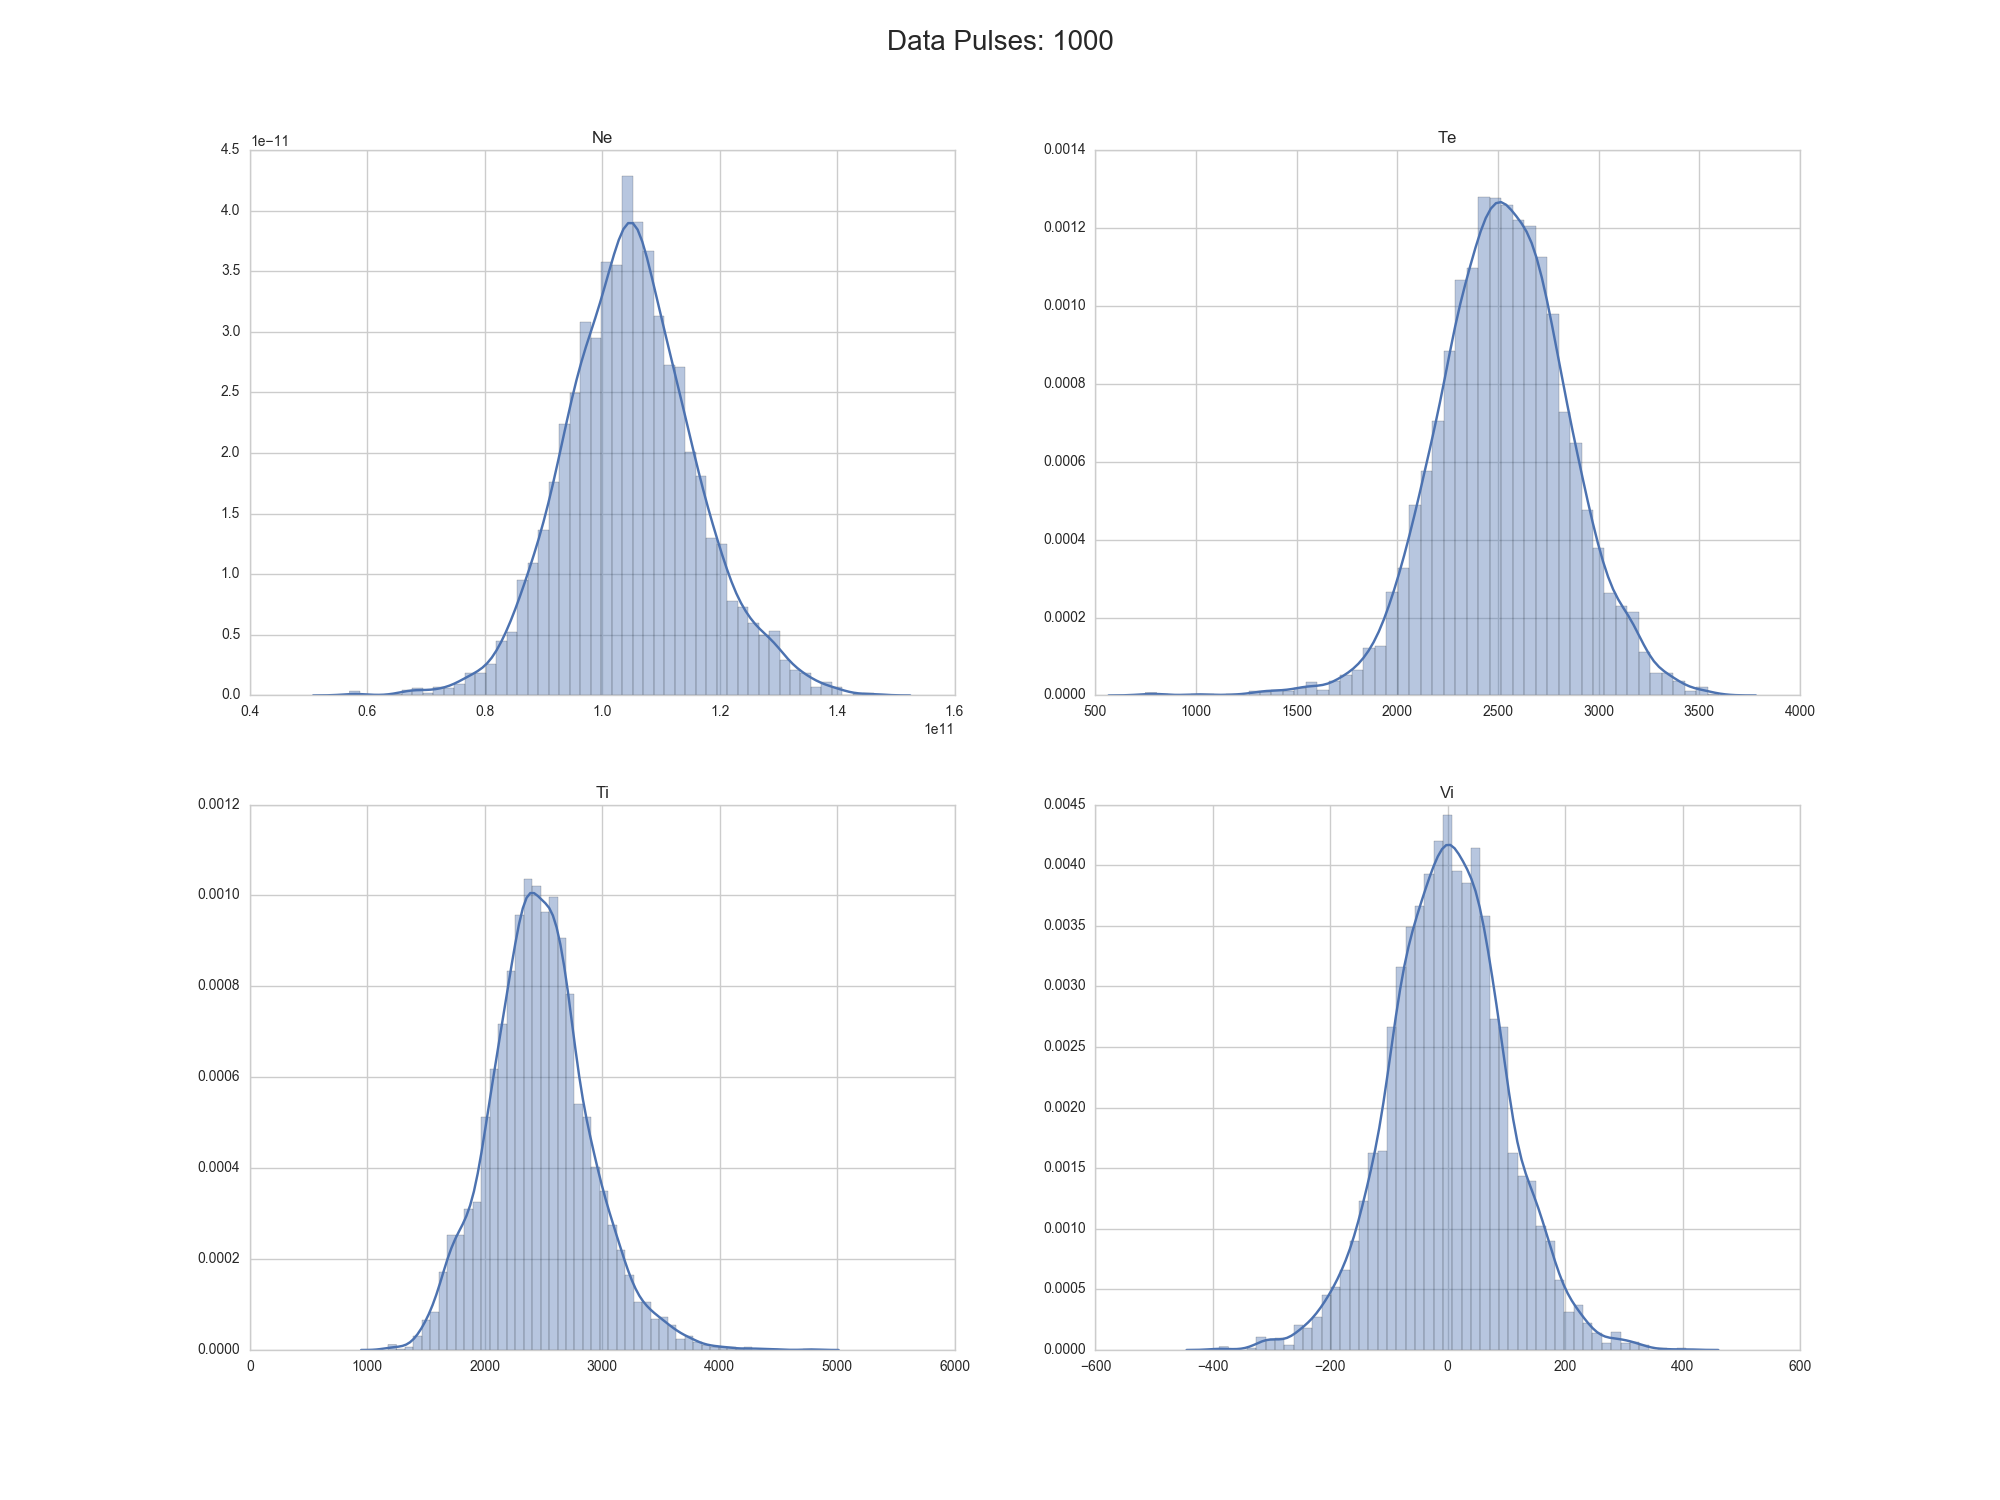
\includegraphics[width=5in]{Data01000pulses}
\caption{Distribution of fitted plasma measurements from cases with 1000 pulses integrated. The bars are histograms and the blue lines Gaussian Kernel Density estimate of the distribution.}
\label{fig:statsdata}
\end{figure}

One can study the observability  of different plasma phenomena with the simulator as well. This can also be done to determine the best experiment set up. In order to show plasma parameters derived from a multi-fluid model developed in \cite{semeter:plasmatransport2012} are used to drive the simulator. The specific example was originally used in \cite{Perry:2015jf} to compare to measurements from RISR-N. Images of the plasma parameters can be seen in Figures \ref{fig:plparamst0}, \ref{fig:plparamst60} and \ref{fig:plparamst120}.


\begin{figure}[!t]
\centering
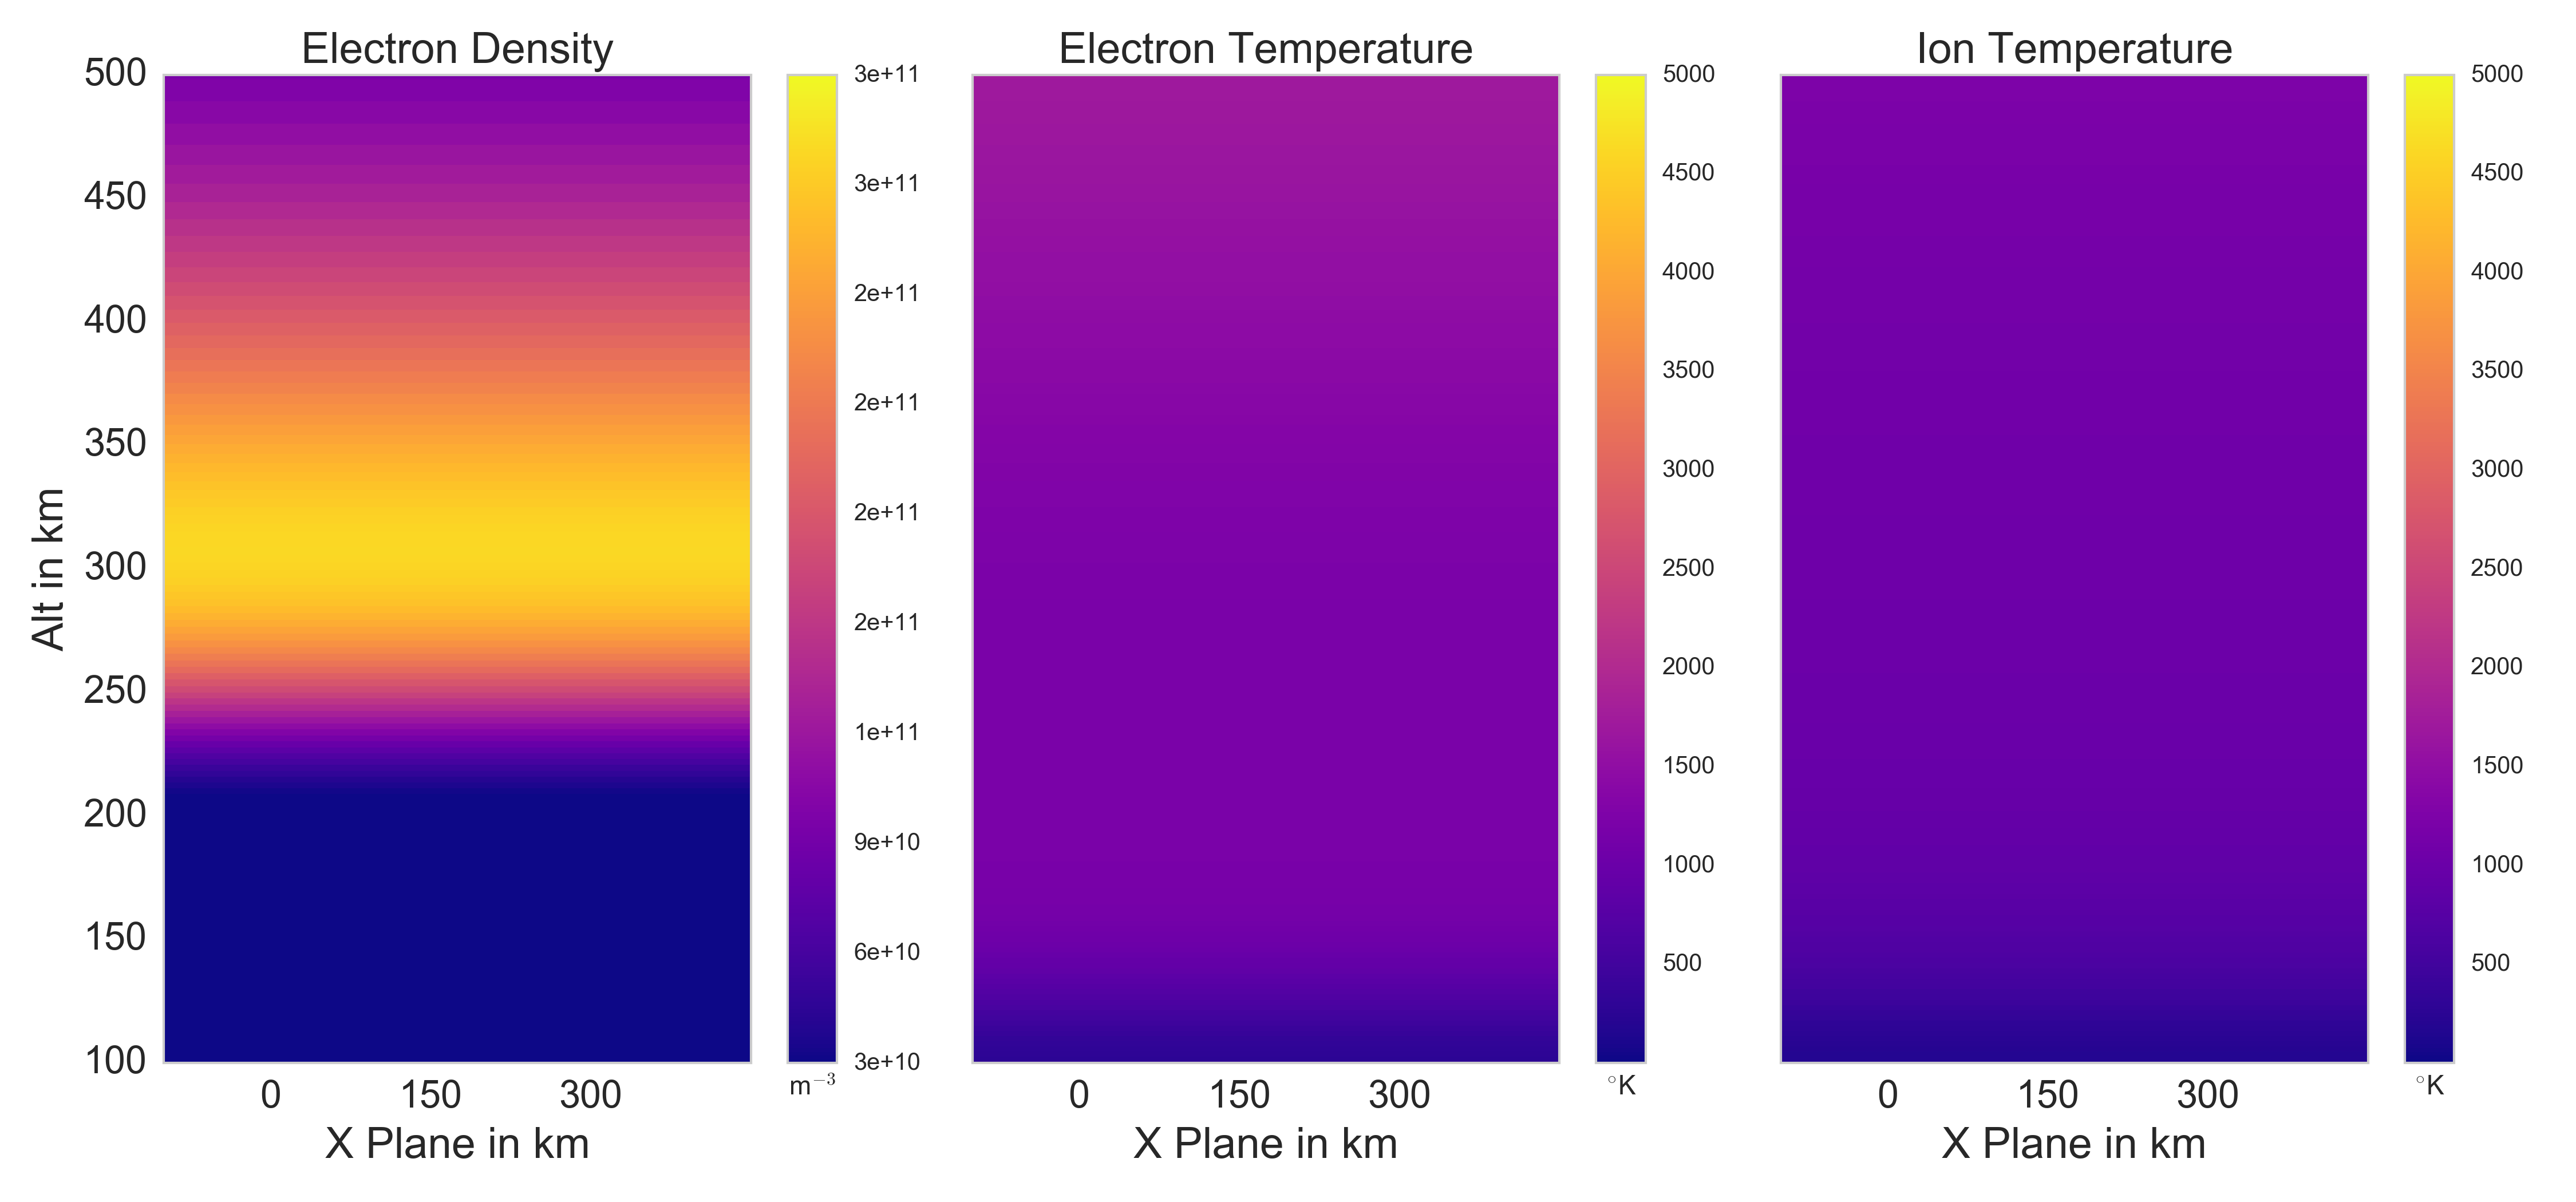
\includegraphics[width=5in]{000_inputdata}
\caption{Plasma Parameters at $t=18000$ s}
\label{fig:plparamst0}
\end{figure}

\begin{figure}[!t]
\centering
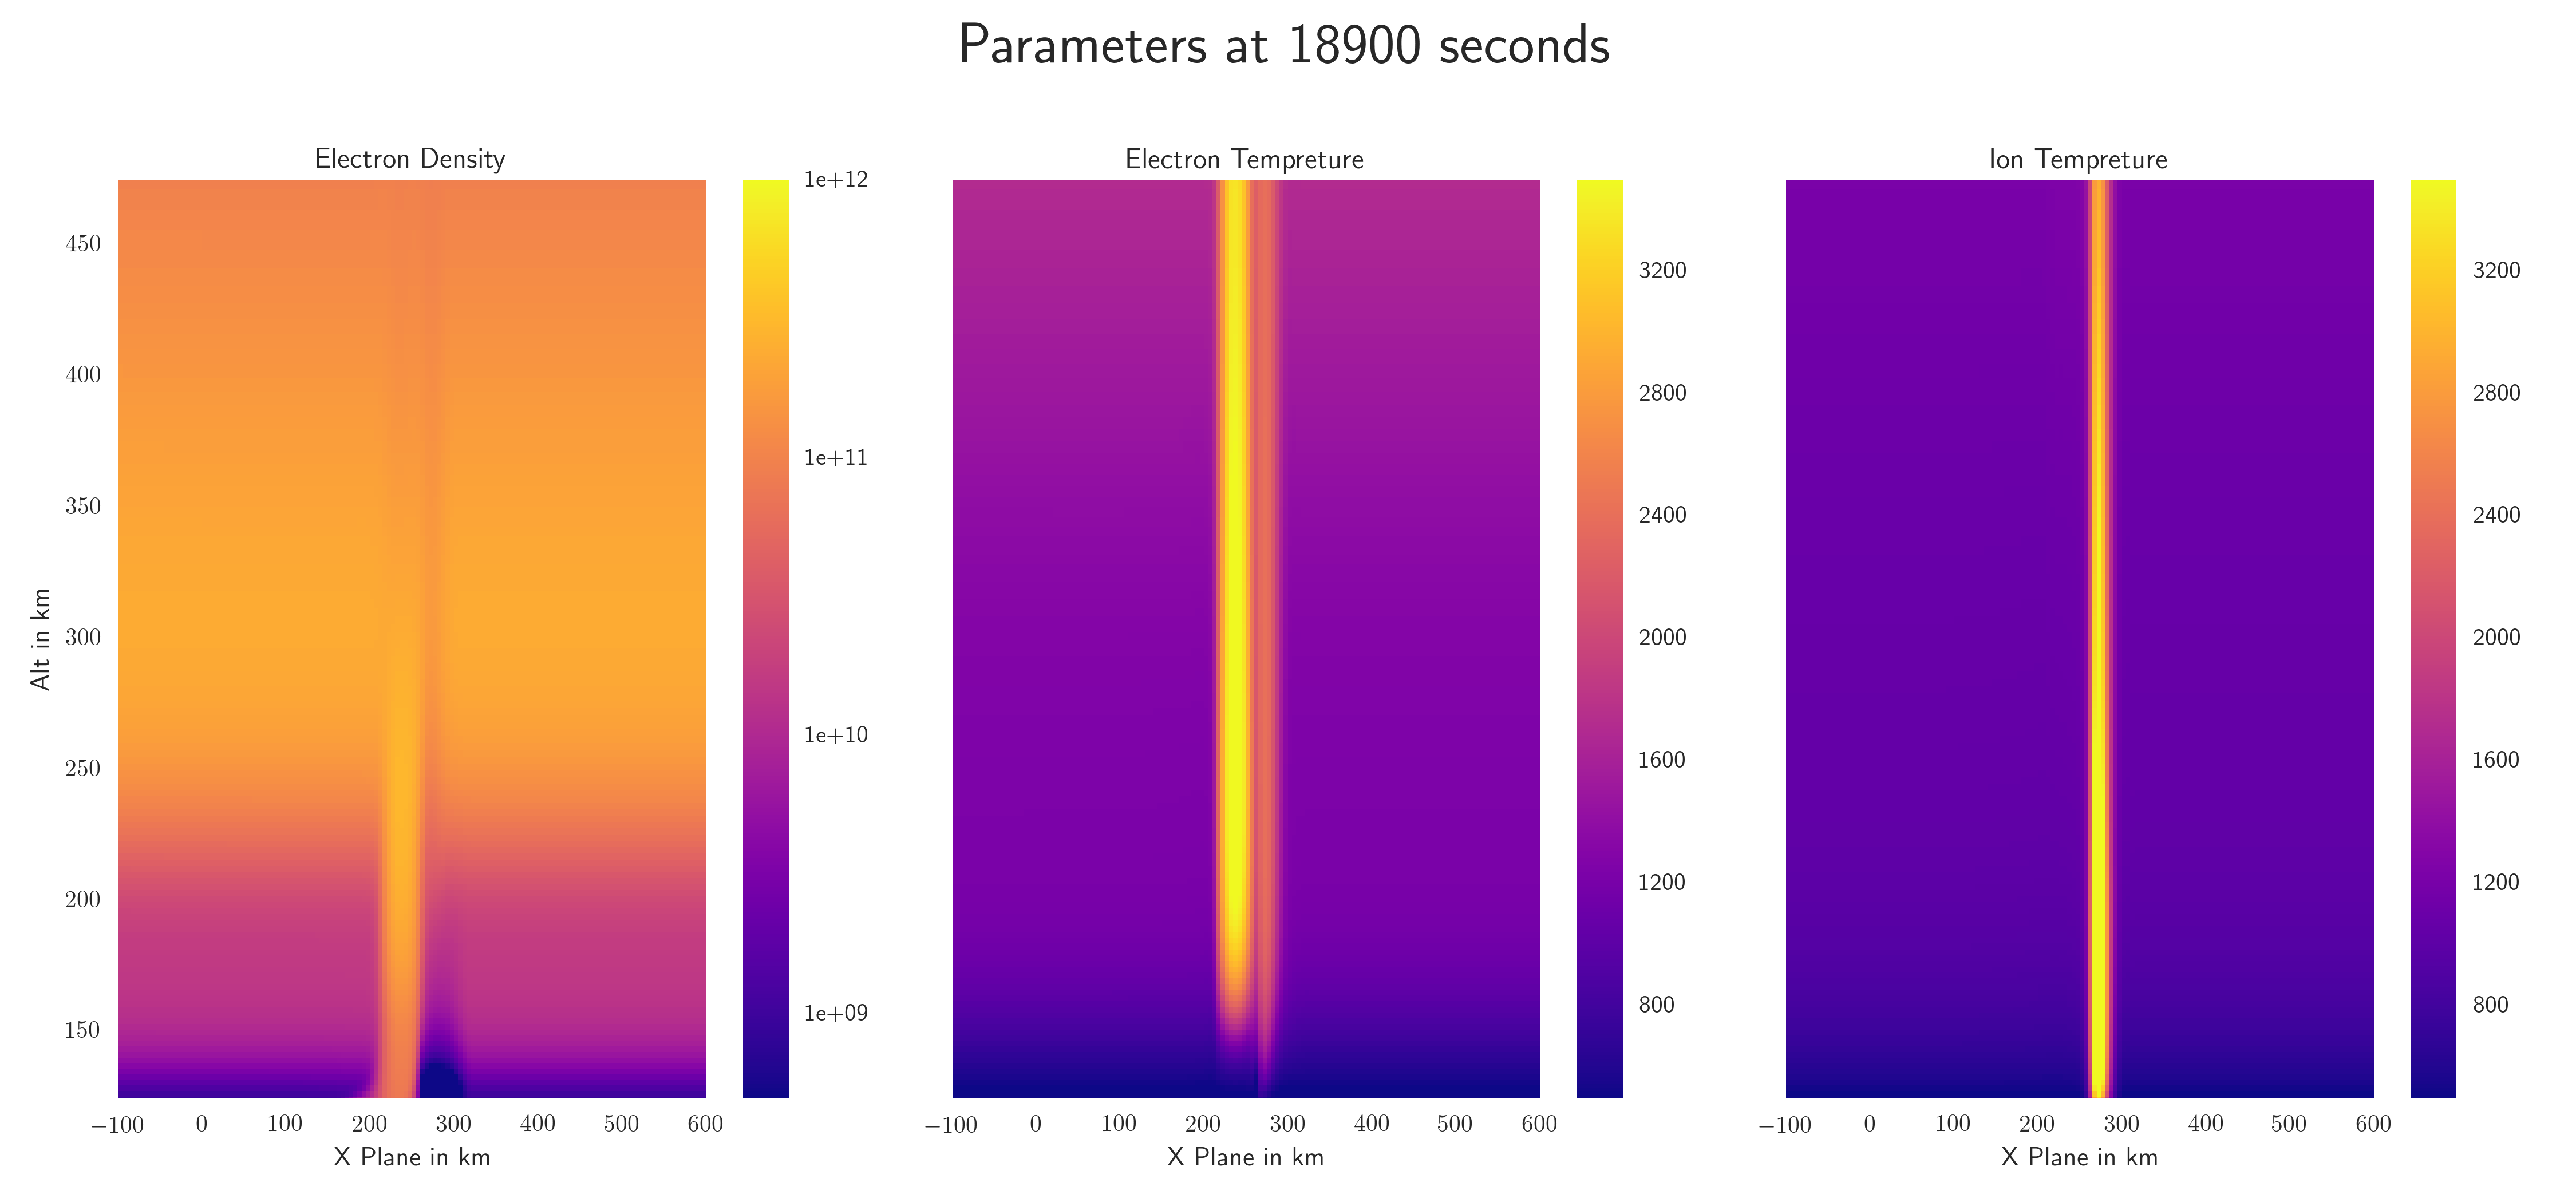
\includegraphics[width=5in]{060_inputdata}
\caption{Plasma Parameters at $t=18900$ s}
\label{fig:plparamst60}
\end{figure}


\begin{figure}[!t]
\centering
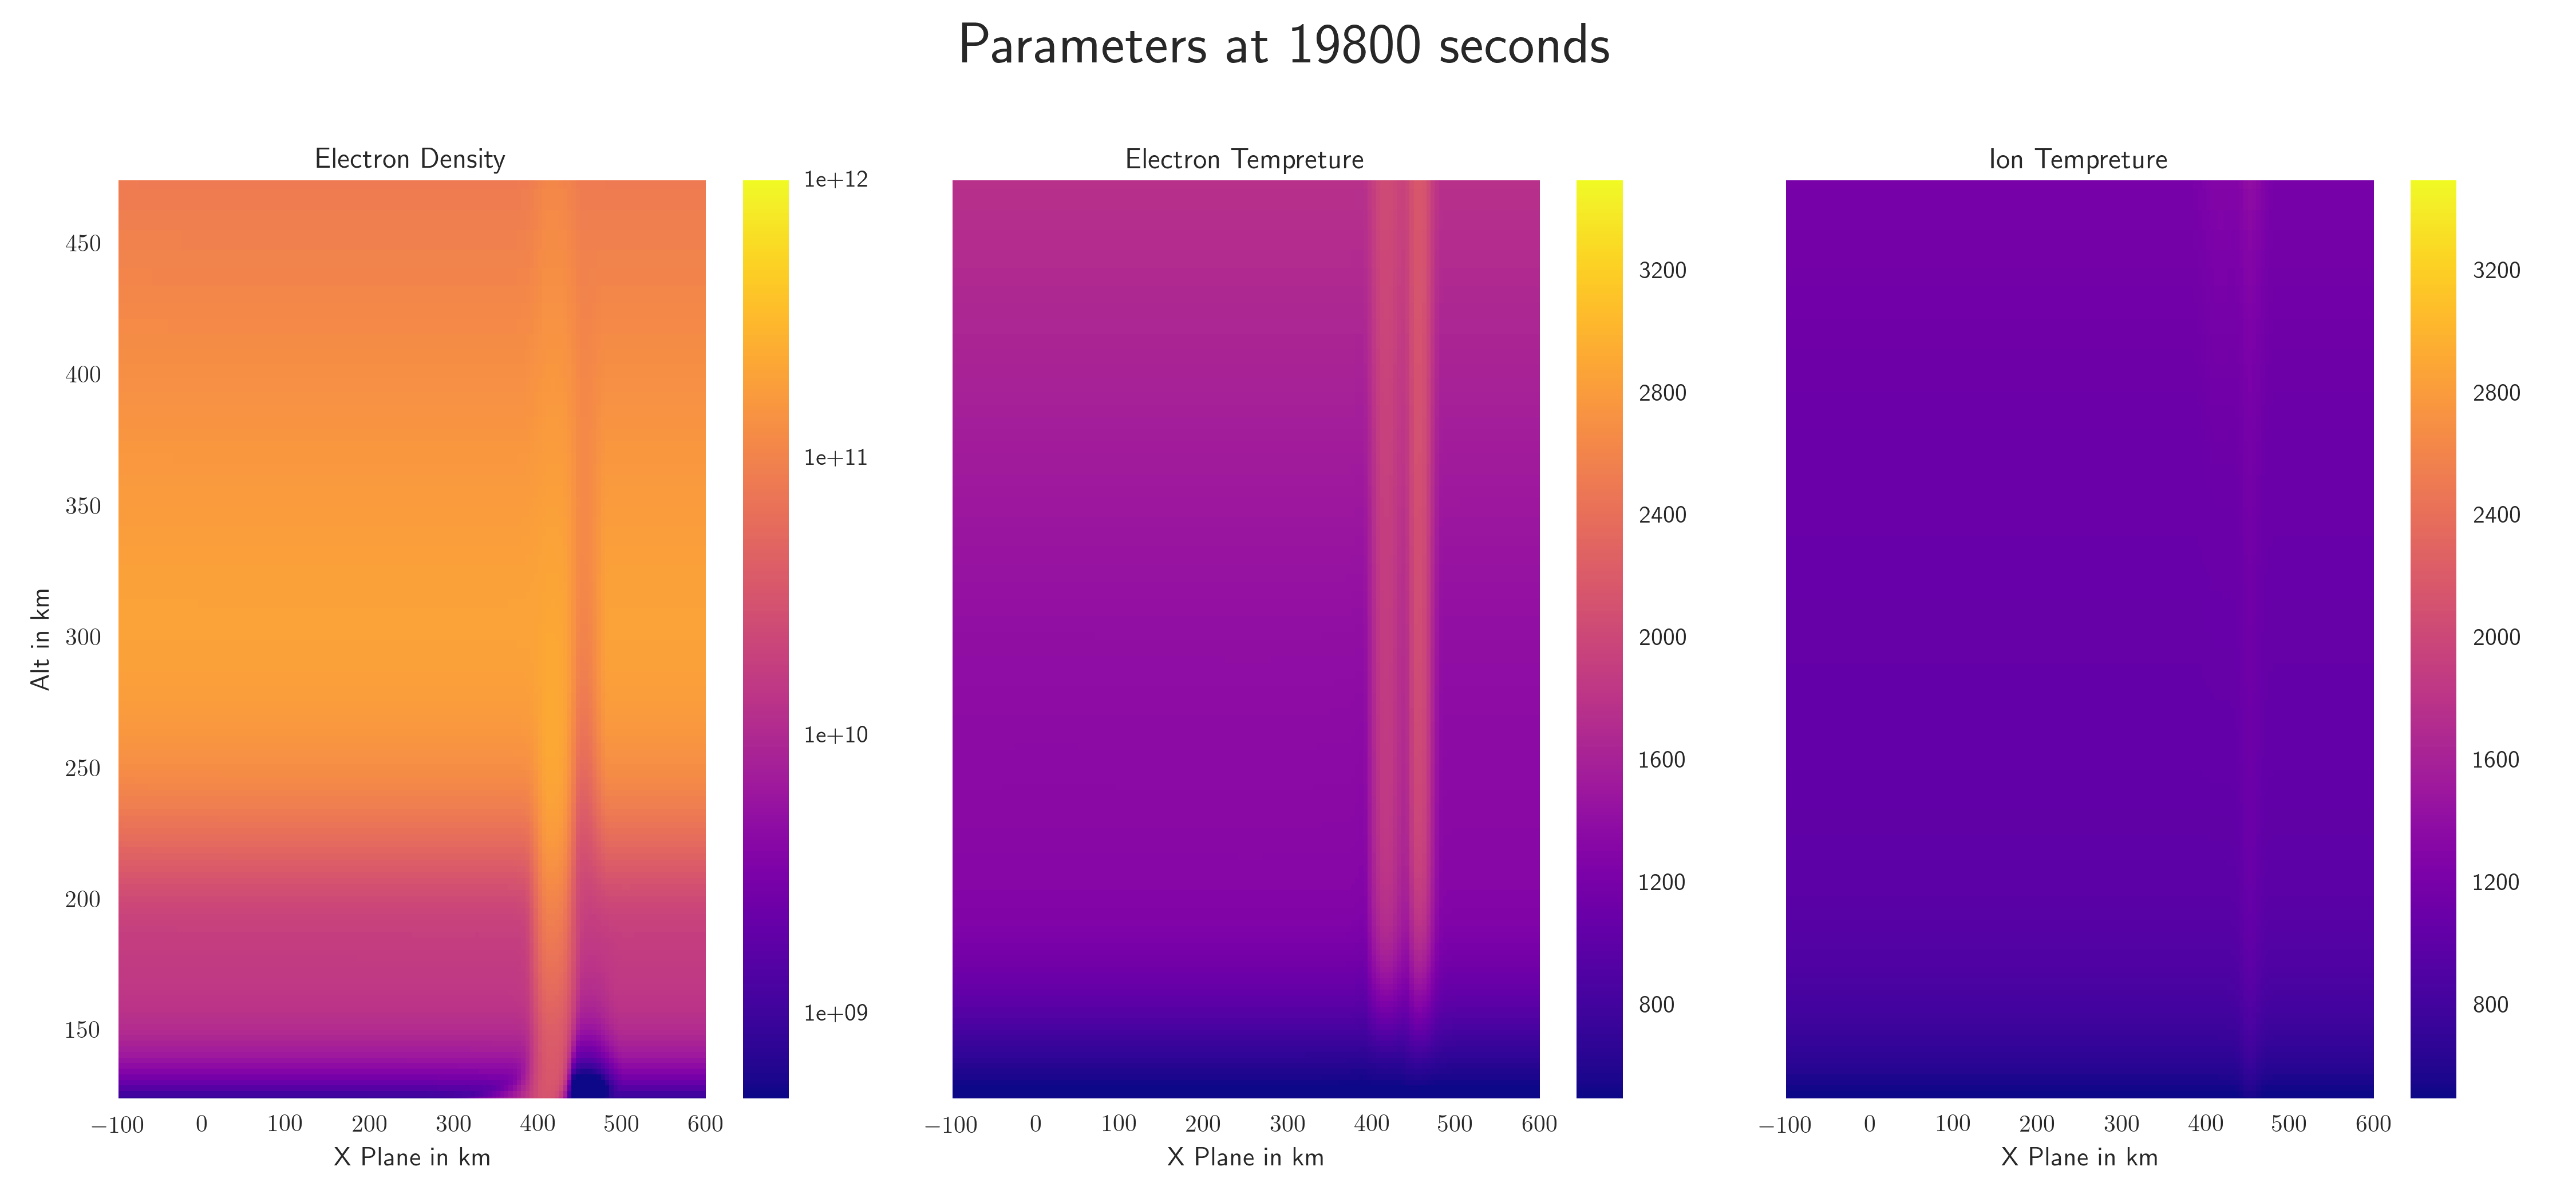
\includegraphics[width=5in]{120_inputdata}
\caption{Plasma Parameters at $t=19800$ s}
\label{fig:plparamst120}
\end{figure}

The output of the ISR simulator from the parameters can be see in Figures \ref{fig:fplparamst0}, \ref{fig:fplparamst60} and \ref{fig:fplparamst120}. This simulation shows a 60 second integration time, which for the 27 beam experiment set up gives 255 pulses per position. The depletion in electron density can still be observed in some of the figures.

%% Fitted Data
\begin{figure}[!t]
\centering
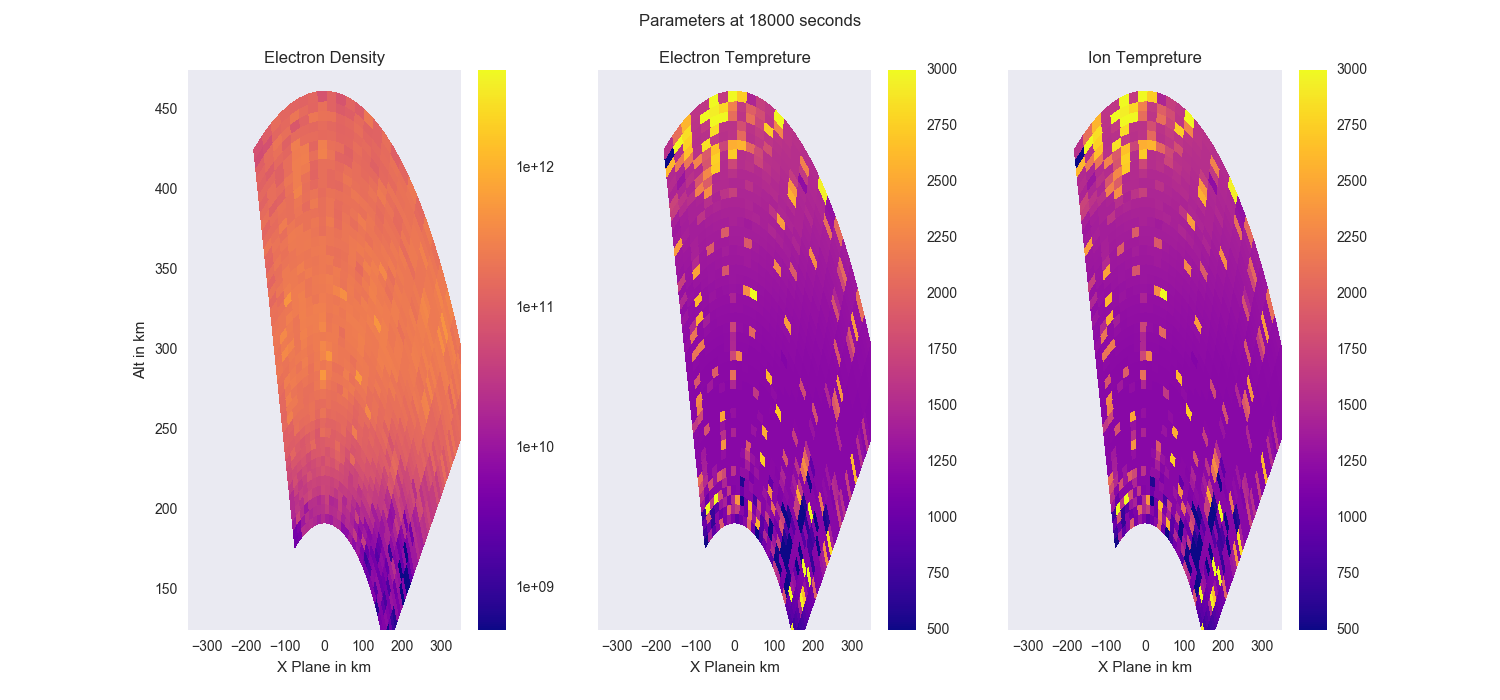
\includegraphics[width=5in]{000_fitteddata}
\caption{Fitted Plasma Parameters at $t=18000$ s}
\label{fig:fplparamst0}
\end{figure}

\begin{figure}[!t]
\centering
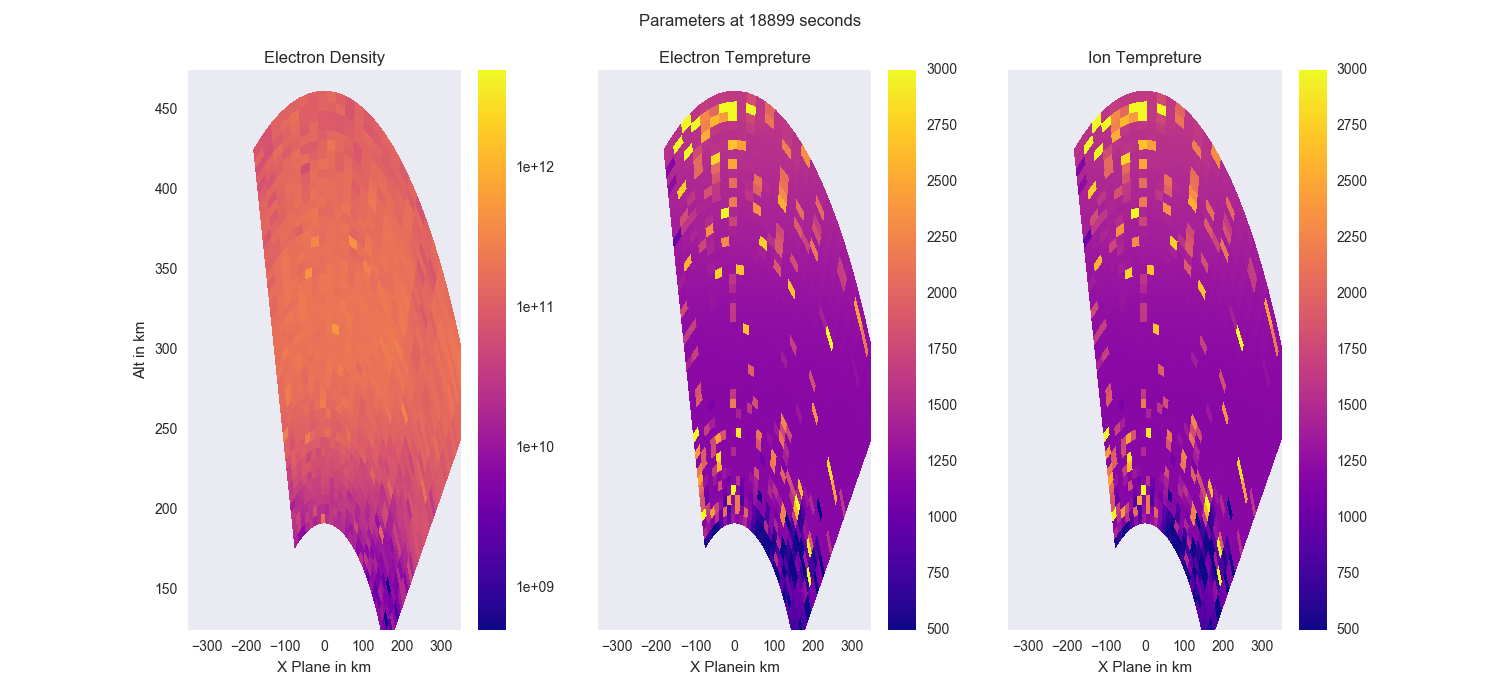
\includegraphics[width=5in]{015_fitteddata}
\caption{Fitted Plasma Parameters at $t=18900$ s}
\label{fig:fplparamst60}
\end{figure}


\begin{figure}[!t]
\centering
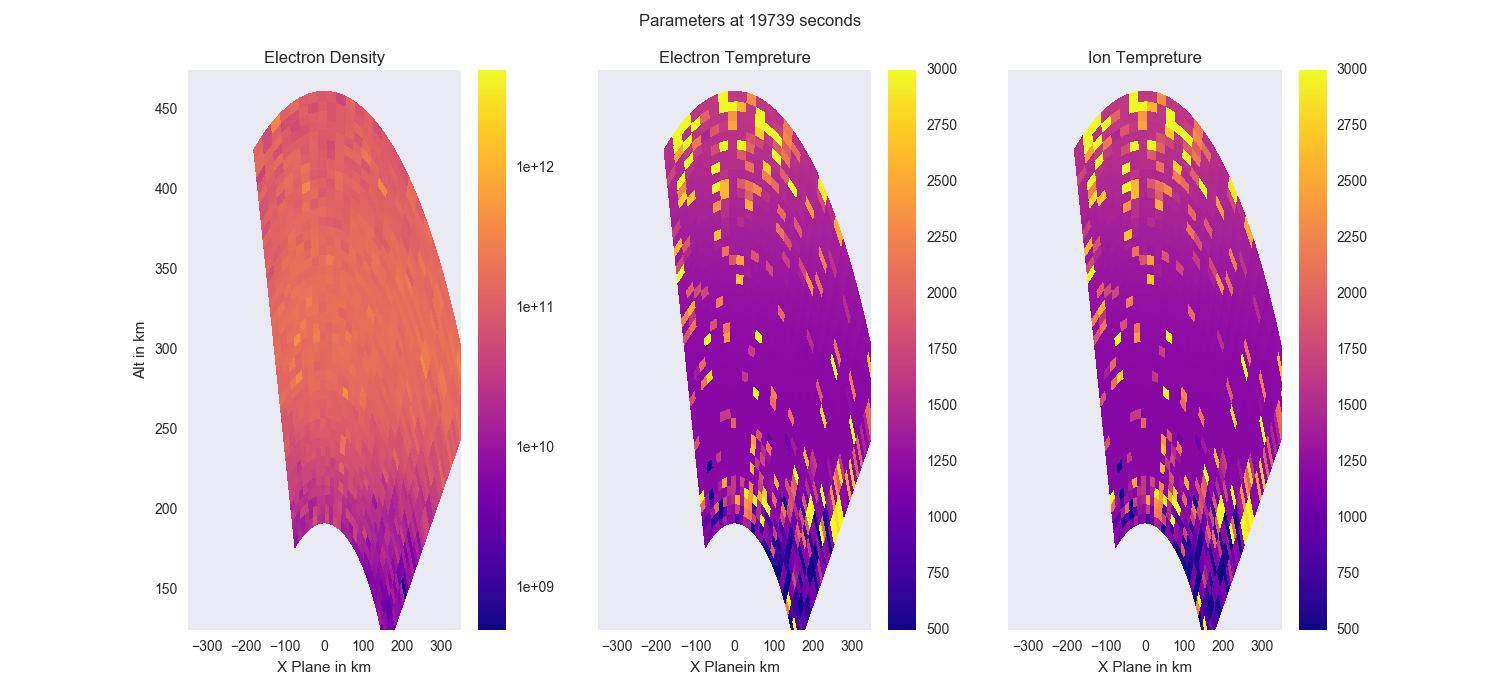
\includegraphics[width=5in]{029_fitteddata}
\caption{Fitted Plasma Parameters at $t=19740$ s}
\label{fig:fplparamst120}
\end{figure}


%%%%%%%%%%%%%%%%%%%%%%%%%%%%%%%%%%%%%%%%%%%%%%%%%%%%%%%%%%%%%%%%%%%%%%%%%%%%%%%%%%%%%%%%%%
\section{Conclusion}
Sources of error in the ISR measurement process have be discussed along with the description of a full simulation of the measurement process. Possible uses for the simulator in research community have also been discussed and examples have been show. The simulator can help researchers plan their experiments and help understand the statistical errors that may arise from their experiments. 

%%%%%%%%%%%%%%%%%%%%%%%%%%%%%%%%%%%%%%%%%%%%%%%%%%%%%%%%%%%%%%%%%%%%%%%%%%%%%%%%%%%%%%%%%%
\begin{acknowledgments}
This work was supported by the National Science Foundation, through Aeronomy Program Grant AGS-1339500 to Boston University and Cooperative Agreement AGS-1242204 between the NSF and the Massachusetts Institute of Technology, and by the Air Force Office of Scientific Research under contract FA9550-12-1-018.   The authors are grateful to the International Space Science Institute (ISSI, Bern, Switzerland) for sponsoring a series of workshops from which the idea for this work emerged. 

Software used to create figures for this publications can be found at https://github.com/jswoboda/. Please contact the corresponding author, John Swoboda at swoboj@bu.edu, with any questions regarding the software along with any requests for the specific data used for the figures. \end{acknowledgments}


\bibliographystyle{BibTeX/agufull08}
\bibliography{BibTeX/litreview}
\end{article}

\end{document}

